%11_graphs.tex
%notes for the course PandA2 COMS10001 taught at the University of Bristol
%2016-7 Conor Houghton conor.houghton@bristol.ac.uk

%To the extent possible under law, the author has dedicated all copyright 
%and related and neighboring rights to these notes to the public domain 
%worldwide. These notes are distributed without any warranty. 

\documentclass[11pt,a4paper]{scrartcl}
\typearea{12}
\usepackage{graphicx}
\usepackage{listings}
\usepackage{tikz}
%\usepackage{tikz-qtree}                                                        
\usetikzlibrary{positioning}
\usetikzlibrary{arrows.meta}
\lstset{language=C}
\pagestyle{headings}
\markright{COMS10001 - PandA2 11\_graphs - Conor}
\begin{document}

\subsection*{11- graphs\footnote{\texttt{http://github.com/conorhoughton/COMS10001}} - UNFINISHED}

Graphs are a useful way to represent data; there are powerful
algorithms for graphs and so by describing some type data as a graph
it becomes possible to process it using these algorithms. From a more
theoretical point-of-view, graphs present interesting problems to the
study of algorithms and some branches of mathematics, like
combinatorics; many graph theory problems have interesting and elegant
solutions while others are unsolved.

A graph is a set \textsl{nodes}, also called \textsl{vertices} linked
by \textsl{edges}. In an undirected graph, these edges have no
direction, as in Fig.~\ref{fig:graph}, in a directed graph, the edges
have direction, as in Fig.~\ref{fig:dir_graph} and in a weighted graph
the edges have a weight, as in Fig.~\ref{fig:wei_graph}. Facebook is
an undirected graph, since \lq{}friendship\rq{} is reciprocal, Twitter
is an directed graph since \lq{}following\rq{} is not reciprocal; the
distances between cities connected by train lines is weighted
graph. You can imagine other possibilities, like directed weighted
graphs and graphs where the nodes also have weights, but we will only
consider directed, undirected and weighted here.

A common way to describe a graph algebraically is to use the adjacency
matrix. This describes the connections between the nodes; for an undirected graph it is the matrix:
\begin{equation}
A_{ij}=\left\{\begin{array}{cl}1&i\mbox{ is connected to }j\cr0&\mbox{otherwise}
\end{array}\right.
\end{equation}
so there is a one in the matrix in the $i$th row and $j$th column if
the $i$th node is connected to the $j$th node. The graphs we have
drawn all have letters labeling the nodes, so obviously for the matrix
you need to number the nodes, here we'll just make $a$ node 1, $b$ node two and so on, with this adjacency matrix for the graph in Fig.~\ref{fig:graph} is
\begin{equation}
A=[A_{ij}]=\left(
\begin{array}{ccccc}
0&1&1&1&0\\
1&0&1&0&0\\
1&1&0&1&0\\
1&0&1&0&1\\
0&0&0&1&0
\end{array}
\right)
\end{equation}



\begin{figure}
\begin{center}
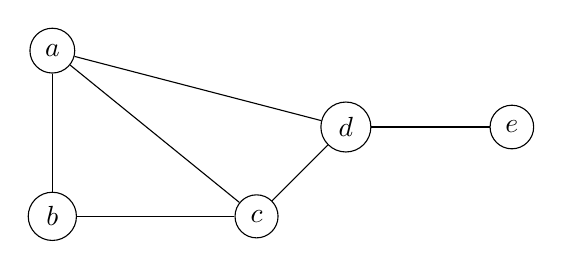
\begin{tikzpicture}
\node[draw,circle](a){$a$};
\node[draw,circle, below = 1.5cm of a](b){$b$};
\node[draw,circle, right =2cm of b](c){$c$};
\node[draw,circle, above right = 1cm of c](d){$d$};
\node[draw,circle, right = 1.5cm of d](e){$e$};
\path (a) edge (b);
\path (b) edge (c);
\path (c) edge (d);
\path (d) edge (e);
\path (a) edge (d);
\path (c) edge (a);
\end{tikzpicture}
\end{center}
\caption{A graph: this is an undirected graph so the edges have no
  direction. \label{fig:graph}}
\end{figure}

For a directed graph there is a one in the $i$th row and $j$ column of the adjacency matrix if there is a link from $i$ to $j$, so it is the matrix:
\begin{equation}
A_{ij}=\left\{\begin{array}{cl}1&i\mbox{ has an edge pointing to }j\cr0&\mbox{otherwise}
\end{array}\right.
\end{equation}
so, in the case of Fig.~\ref{fig:dir_graph} the matrix is 
\begin{equation}
A=\left(
\begin{array}{ccccc}
0&1&0&1&0\\
1&0&1&0&0\\
1&0&0&1&0\\
0&0&0&0&1\\
0&0&0&1&0
\end{array}
\right)
\end{equation}
In the weighted graph, as you might expect, the matrix entries correspond to the weights, so
\begin{equation}
A_{ij}=\left\{
\begin{array}{cl}
w&i\mbox{ is connected with weight }w\mbox{ to }j\cr 
0&\mbox{otherwise}
\end{array}\right.
\end{equation}
so the matrix is
\begin{equation}
A=\left(
\begin{array}{ccccc}
0&5&6&3&0\\
5&0&2&0&0\\
6&2&0&8&0\\
3&0&8&0&1\\
0&0&0&1&0
\end{array}
\right)
\end{equation}


\begin{figure}
\begin{center}
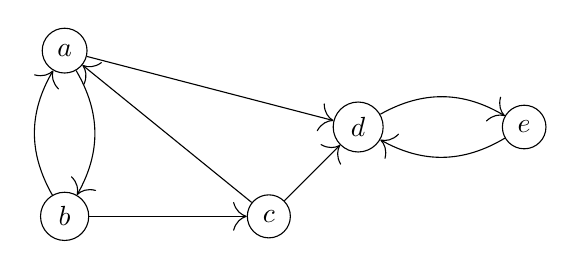
\begin{tikzpicture}
\node[draw,circle](a){$a$};
\node[draw,circle, below = 1.5cm of a](b){$b$};
\node[draw,circle, right =2cm of b](c){$c$};
\node[draw,circle, above right = 1cm of c](d){$d$};
\node[draw,circle, right = 1.5cm of d](e){$e$};
\path (a) edge[-{>[scale=2]},bend left] (b);
\path (b) edge[-{>[scale=2]},bend left] (a);
\path (b) edge[-{>[scale=2]}] (c);
\path (c) edge[-{>[scale=2]}] (d);
\path (d) edge[-{>[scale=2]},bend left] (e);
\path (e) edge[-{>[scale=2]},bend left] (d);
\path (a) edge[-{>[scale=2]}] (d);
\path (c) edge[-{>[scale=2]}] (a);
\end{tikzpicture}
\end{center}
\caption{A directed graph. \label{fig:dir_graph}}
\end{figure}


\begin{figure}
\begin{center}
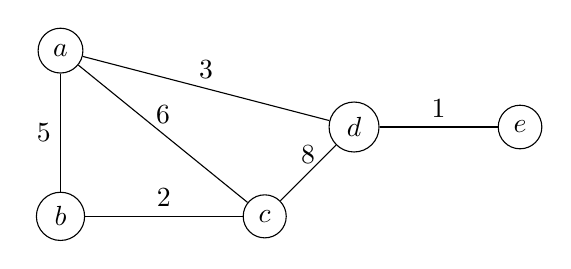
\begin{tikzpicture}
\node[draw,circle](a){$a$};
\node[draw,circle, below = 1.5cm of a](b){$b$};
\node[draw,circle, right =2cm of b](c){$c$};
\node[draw,circle, above right = 1cm of c](d){$d$};
\node[draw,circle, right = 1.5cm of d](e){$e$};
\path (a) edge node[left]{5} (b);
\path (b) edge node[above]{2} (c);
\path (c) edge  node[above]{8}(d);
\path (d) edge  node[above]{1}(e);
\path (a) edge  node[above]{3}(d);
\path (c) edge  node[above]{6}(a);
\end{tikzpicture}
\end{center}
\caption{A graph: this is a weighted graph so the edges have a value. \label{fig:wei_graph}}
\end{figure}



\begin{figure}
\begin{center}
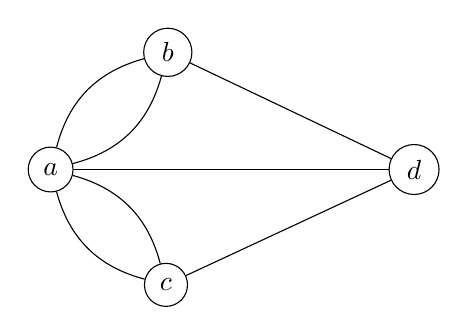
\begin{tikzpicture}
\node[draw,circle](a){$a$};
\node[draw,circle, above right = 1.5cm of a](b){$b$};
\node[draw,circle, below right = 1.5 cm of a](c){$c$};
\node[draw,circle, right = 4cm of a](d){$d$};
\path (a) edge[-,bend right] (b);
\path (a) edge[-,bend left] (b);
\path (a) edge[-,bend right] (c);
\path (a) edge[-,bend left] (c);
\path (a) edge[-] (d);
\path (d) edge[-] (b);
\path (d) edge[-] (c);
\end{tikzpicture}
\end{center}
\caption{The Bridges of K\"{o}nigsberg graph. \label{fig:konigsberg_graph}}
\end{figure}





\end{document}
